\documentclass[12pt,a4paper]{article}

% ------------------------- Packages -------------------------
\usepackage[margin=1in]{geometry}
\usepackage{graphicx}
\usepackage{float}
\usepackage{booktabs}
\usepackage{tabularx}
\usepackage{array}
\usepackage{longtable}
\usepackage{enumitem}
\usepackage{xcolor}
\usepackage{hyperref}
\usepackage{listings}
\usepackage{caption}
\usepackage{subcaption}
\usepackage{fancyhdr}
\usepackage{titlesec}
\usepackage{tikz}
\usetikzlibrary{arrows.meta,positioning,shapes.geometric,fit}
\usepackage{microtype}
\usepackage{setspace}
\usepackage{parskip}
\usepackage{lastpage}
\usepackage{ifthen}

% ------------------------- Colors -------------------------
\definecolor{navy}{HTML}{17324D}
\definecolor{blueaccent}{HTML}{2F6B9A}
\definecolor{lightblue}{HTML}{EAF2F8}
\definecolor{lightgray}{HTML}{F4F6F7}
\definecolor{darkgray}{HTML}{4D5656}
\definecolor{codegreen}{HTML}{2E7D32}
\definecolor{codepurple}{HTML}{6A1B9A}

% ------------------------- Hyperlinks -------------------------
\hypersetup{
    colorlinks=true,
    linkcolor=navy,
    urlcolor=blueaccent,
    citecolor=navy,
    pdftitle={Lab 4 - Weather Stations Monitoring Technical Report},
    pdfauthor={Ahmed Walaaeldin, Mazen Adel, Marwan Ahmed, Ahmed Ibrahim}
}

% ------------------------- Headings -------------------------
\titleformat{\section}
  {\Large\bfseries\color{navy}}
  {\thesection}{0.7em}{}
\titleformat{\subsection}
  {\large\bfseries\color{blueaccent}}
  {\thesubsection}{0.6em}{}
\titleformat{\subsubsection}
  {\normalsize\bfseries\color{darkgray}}
  {\thesubsubsection}{0.5em}{}

% ------------------------- Header / Footer -------------------------
\pagestyle{fancy}
\setlength{\headheight}{14pt}
\fancyhf{}
\fancyhead[L]{\small Net Centric Computing - Lab 4}
\fancyhead[R]{\small Weather Stations Monitoring}
\fancyfoot[C]{\small Page \thepage\ of \pageref{LastPage}}
\renewcommand{\headrulewidth}{0.4pt}
\renewcommand{\footrulewidth}{0.2pt}

% ------------------------- Listings -------------------------
\lstdefinestyle{code}{
    backgroundcolor=\color{lightgray},
    basicstyle=\ttfamily\small,
    breaklines=true,
    frame=single,
    rulecolor=\color{gray!35},
    numbers=left,
    numberstyle=\tiny\color{gray},
    keywordstyle=\color{blueaccent}\bfseries,
    commentstyle=\color{codegreen},
    stringstyle=\color{codepurple},
    showstringspaces=false,
    tabsize=2,
    columns=fullflexible
}
\lstset{style=code}

% ------------------------- Figure helper -------------------------
% This lets the report compile even if an optional screenshot is missing.
\newcommand{\reportfigure}[3]{%
\begin{figure}[H]
    \centering
    \IfFileExists{#1}{%
        \includegraphics[width=#2\textwidth,height=0.72\textheight,keepaspectratio]{#1}%
    }{%
        \fbox{\parbox[c][4cm][c]{0.86\textwidth}{\centering\textbf{Screenshot placeholder}\\[0.5em]\texttt{#1}}}%
    }
    \caption{#3}
\end{figure}
}


% ------------------------- Document metadata -------------------------
\newcommand{\coursename}{Net Centric Computing}
\newcommand{\labtitle}{Lab 4 - Weather Stations Monitoring}
\newcommand{\academicyear}{Fall 2025--2026}
\newcommand{\faculty}{Faculty of Engineering - Alexandria University}
\newcommand{\department}{Computer and Communications Engineering}

\newcommand{\submissiondate}{\today}

\begin{document}

% ================================================================
% Title Page
% ================================================================
\begin{titlepage}
    \centering
    \vspace*{1.2cm}
    {\Large\bfseries \faculty\par}
    \vspace{0.25cm}
    {\large \department\par}
    \vspace{1.4cm}

    {\Huge\bfseries\color{navy} \labtitle\par}
    \vspace{0.45cm}
    {\Large\color{blueaccent} Technical Report\par}
    \vspace{1.0cm}

    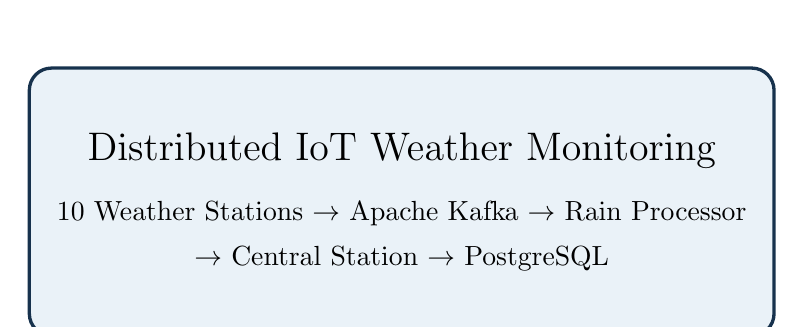
\begin{tikzpicture}
        \node[draw=navy, very thick, rounded corners=8pt, fill=lightblue,
              minimum width=0.78\textwidth, minimum height=3.4cm, align=center] {
            \Large Distributed IoT Weather Monitoring\\[0.35cm]
            \normalsize 10 Weather Stations $\rightarrow$ Apache Kafka $\rightarrow$ Rain Processor\\[0.15cm]
            $\rightarrow$ Central Station $\rightarrow$ PostgreSQL
        };
    \end{tikzpicture}

    \vfill
    \begin{tabular}{>{\bfseries}l l}
        Course: & \coursename \\
        Academic Year: & \academicyear \\
        Date: & \submissiondate \\
    \end{tabular}

    \vspace{0.8cm}
    {\large\bfseries Team Members\par}
    \vspace{0.3cm}
    \begin{tabular}{l r}
        \toprule
        \textbf{Name} & \textbf{ID} \\
        \midrule
        Ahmed Walaaeldin & 8625 \\
        Mazen Adel & 8634 \\
        Marwan Ahmed & 8824 \\
        Ahmed Ibrahim & 8672 \\
        \bottomrule
    \end{tabular}
    \vfill
\end{titlepage}

\tableofcontents
\newpage
\listoffigures
\newpage

% ================================================================
\section{Introduction}
% ================================================================
The objective of this lab is to design and implement a distributed weather monitoring system that models a practical Internet of Things (IoT) stream-processing pipeline. Multiple weather stations continuously generate readings, Apache Kafka provides asynchronous transport and buffering, a Kafka Streams processor detects special weather conditions, and a central station persists historical data to a relational SQL database.

The implemented system follows the required architecture while adding reliability and deployment considerations. Ten independent weather station services emit one reading per second. Each generated reading contains a station identifier, a per-station sequence number, battery status, timestamp, humidity, temperature, and wind speed. Approximately 10\% of generated messages are intentionally dropped to simulate unreliable sensing or transmission. The battery status is sampled to converge statistically toward a 30\% low, 40\% medium, and 30\% high distribution.

Apache Kafka decouples producers from downstream processing. Weather readings are published to the \texttt{weather-readings} topic, while a Kafka Streams processor identifies readings with humidity greater than 70\% and publishes a special alert to \texttt{rain-alerts}. The central station consumes the streams and writes them to PostgreSQL. Weather readings are inserted using JDBC batches to reduce database I/O, and the application commits Kafka offsets only after the corresponding database transaction succeeds.

The system was first validated locally, then deployed on Kubernetes using Minikube. The bonus deployment separates weather stations from the central base station across cloud virtual machines and uses an externally managed PostgreSQL database.

% ================================================================
\section{System Architecture}
% ================================================================
\subsection{High-Level Design}

\begin{figure}[H]
\centering
\resizebox{0.94\textwidth}{!}{%
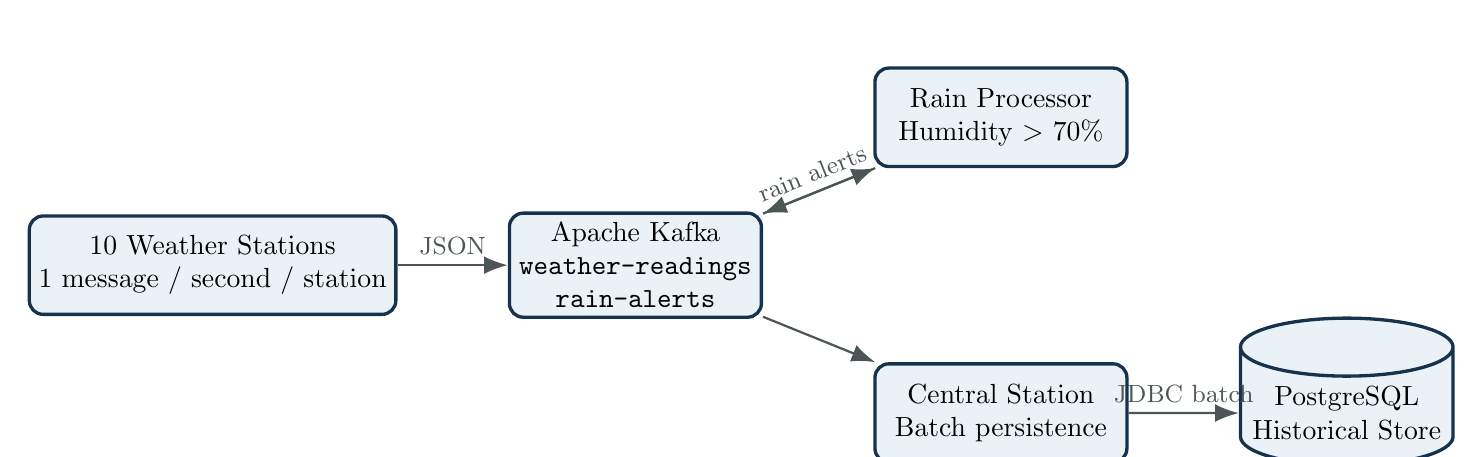
\begin{tikzpicture}[
    node distance=1.2cm and 1.4cm,
    box/.style={draw=navy, very thick, rounded corners=5pt, fill=lightblue,
                align=center, minimum height=1.25cm, minimum width=3.2cm},
    db/.style={draw=navy, very thick, cylinder, shape border rotate=90,
               aspect=0.28, fill=lightblue, minimum height=1.5cm, minimum width=2.7cm, align=center},
    arrow/.style={-{Latex[length=3mm]}, thick, color=darkgray}
]
    \node[box] (stations) {10 Weather Stations\\1 message / second / station};
    \node[box, right=of stations] (kafka) {Apache Kafka\\\texttt{weather-readings}\\\texttt{rain-alerts}};
    \node[box, above right=0.55cm and 1.4cm of kafka] (rain) {Rain Processor\\Humidity $>$ 70\%};
    \node[box, below right=0.55cm and 1.4cm of kafka] (central) {Central Station\\Batch persistence};
    \node[db, right=of central] (db) {PostgreSQL\\Historical Store};

    \draw[arrow] (stations) -- node[above, font=\small]{JSON} (kafka);
    \draw[arrow] (kafka) -- (rain);
    \draw[arrow] (rain) -- node[above, sloped, font=\small]{rain alerts} (kafka);
    \draw[arrow] (kafka) -- (central);
    \draw[arrow] (central) -- node[above, font=\small]{JDBC batch} (db);
\end{tikzpicture}%
}
\caption{Implemented distributed weather monitoring architecture.}
\end{figure}

The architecture is divided into three main stages:
\begin{enumerate}[label=\arabic*.]
    \item \textbf{Data acquisition:} ten weather station services generate simulated sensor readings and publish them to Kafka.
    \item \textbf{Data processing:} Kafka buffers the readings, while the rain processor filters and transforms readings with humidity above the configured threshold.
    \item \textbf{Data persistence and analysis:} the central station stores readings and rain alerts in PostgreSQL, from which historical validation queries are executed.
\end{enumerate}

Kafka is placed between acquisition and processing to provide loose coupling, buffering, replay capability, partition-based ordering, and independent scaling of producers and consumers.

\subsection{Repository Organization}
The implementation is structured as a Maven multi-module project. The \texttt{common} module provides shared message classes and configuration helpers. Separate modules implement the weather stations, rain processor, and central station. Deployment assets are organized into Docker, Kubernetes, SQL, and cloud-specific directories.

\reportfigure{images/18-project-structure.png}{0.96}{Project repository structure.}

\begin{table}[H]
\centering
\caption{Main repository components.}
\begin{tabularx}{\textwidth}{>{\ttfamily}l X}
\toprule
\textbf{Path} & \textbf{Purpose} \\
\midrule
common/ & Shared JSON models, Kafka topic names, and environment-based configuration helpers. \\
weather-station/ & Parts A and B: reading generation and Kafka production. \\
rain-processor/ & Part C: Kafka Streams rain detection using the Processor API, plus a DSL alternative. \\
central-station/ & Part D: Kafka consumers, JDBC batching, and database initialization. \\
sql/ & Part E: relational schema and historical analysis queries. \\
k8s/ & Part F: Kubernetes manifests and deployment script. \\
cloud/ & Bonus: split two-VM deployment and managed PostgreSQL configuration. \\
\bottomrule
\end{tabularx}
\end{table}

% ================================================================
\section{Weather Station Mock - Part A}
% ================================================================
\subsection{Reading Generation}
Each weather station generates one \texttt{WeatherMessage} every second. The station identity is either supplied explicitly using the \texttt{STATION\_ID} environment variable or derived from the ordinal of a Kubernetes StatefulSet pod. This allows pod names \texttt{weather-station-0} through \texttt{weather-station-9} to map automatically to logical station IDs 1 through 10.

The generated message schema is:
\begin{lstlisting}[language={},caption={Weather status JSON schema.}]
{
  "station_id": 1,
  "s_no": 1,
  "battery_status": "low",
  "status_timestamp": 1681521224,
  "weather": {
    "humidity": 35,
    "temperature": 100,
    "wind_speed": 13
  }
}
\end{lstlisting}

The sequence number is incremented for every generated sample \emph{before} the drop decision. Therefore, intentionally dropped messages leave observable gaps in the stored sequence numbers. This design enables Part E to estimate the drop rate directly from the database.

\subsection{Battery Status Distribution}
A single uniform random value in the range $[0,1)$ is used to choose the battery state:
\begin{itemize}
    \item \texttt{low} when $p < 0.30$,
    \item \texttt{medium} when $0.30 \leq p < 0.70$,
    \item \texttt{high} otherwise.
\end{itemize}
This produces the required theoretical distribution of 30\% / 40\% / 30\%, with small deviations expected for finite sample sizes.

\subsection{Simulated Weather and Message Drops}
Humidity is generated uniformly between 0 and 100\%, temperature between 20 and 120 degrees Fahrenheit, and wind speed between 0 and 50 km/h. A second random draw decides whether each generated message is intentionally dropped with probability 0.10. Even if a message is dropped, its sequence number is not reused.

\reportfigure{images/01-weather-station-logs.png}{0.95}{Weather Station 1 logs showing periodic sends and simulated message drops.}

% ================================================================
\section{Kafka Integration - Part B}
% ================================================================
\subsection{Producer Configuration}
The weather station uses the Java Kafka Producer API to publish serialized JSON to the \texttt{weather-readings} topic. The key configuration choices are summarized below.

\begin{table}[H]
\centering
\caption{Weather station Kafka producer configuration.}
\begin{tabularx}{\textwidth}{l l X}
\toprule
\textbf{Property} & \textbf{Value} & \textbf{Reason} \\
\midrule
Bootstrap servers & Environment configured & Supports local, Kubernetes, and cloud deployments. \\
Key serializer & StringSerializer & Station ID is used as the message key. \\
Value serializer & StringSerializer & Weather messages are serialized to JSON strings. \\
\texttt{acks} & \texttt{all} & Improves durability by requiring broker acknowledgement. \\
Idempotence & enabled & Prevents duplicate writes caused by producer retries. \\
Retries & 3 & Handles transient Kafka communication failures. \\
\texttt{linger.ms} & 20 ms & Allows small batching without significantly affecting one-second cadence. \\
Compression & gzip & Reduces network payload size. \\
\bottomrule
\end{tabularx}
\end{table}

\subsection{Partitioning and Ordering}
The Kafka record key is the station ID. Kafka therefore routes all readings from one station consistently to the same partition. This preserves the relative order of messages for each individual station while still allowing records from different stations to be distributed across multiple partitions.

The deployment creates ten partitions for \texttt{weather-readings}, matching the ten logical stations and providing a clear path for parallel downstream processing.

\reportfigure{images/04-kafka-weather-readings.png}{0.98}{Kafka console consumer showing messages from the \texttt{weather-readings} topic.}
\reportfigure{images/10-kafka-topics-list.png}{0.92}{Kafka topics created for weather readings and rain alerts.}

% ================================================================
\section{Rain Detection - Part C}
% ================================================================
\subsection{Kafka Streams Processor API}
The primary rain detection implementation uses the low-level Kafka Streams Processor API. Its topology is conceptually:
\begin{center}
\texttt{weather-readings $\rightarrow$ RainProcessor $\rightarrow$ rain-alerts}
\end{center}

Each incoming record is deserialized into a \texttt{WeatherMessage}. Malformed records are skipped safely. If the weather object is absent or the humidity is less than or equal to 70\%, no downstream record is produced. For readings with humidity greater than 70\%, the processor increments a per-station counter stored in a persistent key-value state store and forwards a \texttt{RainAlert}.

A rain alert contains the original station ID, sequence number, timestamp, humidity, cumulative per-station alert count, and the message \texttt{"It is raining"}.

\subsection{Processor API Versus DSL}
The project also contains an alternative Kafka Streams DSL implementation. The DSL version is concise and expresses the transformation as a stream of \texttt{mapValues}, \texttt{filter}, and \texttt{to} operations. The Processor API version was selected as the primary implementation because it provides explicit control over processor state, state-store access, and record forwarding. This makes the stateful per-station alert counter straightforward to demonstrate.

\reportfigure{images/02-rain-processor-logs.png}{0.95}{Rain processor logs showing humidity values above 70\% being detected.}
\reportfigure{images/05-kafka-rain-alerts.png}{0.98}{Kafka console consumer showing messages from the \texttt{rain-alerts} topic.}

% ================================================================
\section{Central Station - Part D}
% ================================================================
\subsection{Concurrent Consumers}
The central station initializes the database schema and runs two Kafka consumers in separate threads:
\begin{itemize}
    \item a weather readings consumer for \texttt{weather-readings};
    \item a rain alerts consumer for \texttt{rain-alerts}.
\end{itemize}

Separate JDBC connections are used because JDBC connections are not thread-safe. Both consumers use manual Kafka offset commits.

\subsection{Batch Persistence}
The weather readings consumer buffers messages in memory and flushes them to PostgreSQL when either:
\begin{itemize}
    \item the buffer reaches the configured batch size of 5000 records, or
    \item the flush interval of 10 seconds expires while pending records exist.
\end{itemize}

The batch writer uses a prepared statement and JDBC \texttt{executeBatch()} so a group of readings can be persisted in one transaction rather than requiring one network and transaction round trip per row. This significantly reduces database I/O overhead under sustained streaming load.

\subsection{Delivery Semantics and Idempotency}
The persistence sequence is deliberately:
\begin{enumerate}[label=\arabic*.]
    \item write the batch to PostgreSQL;
    \item commit the PostgreSQL transaction;
    \item commit Kafka offsets.
\end{enumerate}

This provides at-least-once delivery. If the process fails after the database commit but before the Kafka offset commit, the same Kafka records may be consumed again after restart. To make such reprocessing harmless, the table enforces \texttt{UNIQUE(station\_id, sequence\_number)} and the insert statement uses \texttt{ON CONFLICT DO NOTHING}. Consequently, re-read records do not produce duplicate historical rows.

\subsection{Database Schema}
The main table stores all weather readings and includes indexes optimized for per-station sequence queries and battery distribution analysis. A second table archives rain alerts. The \texttt{latest\_station\_status} view uses PostgreSQL \texttt{DISTINCT ON} to return the latest sequence for every station.

\begin{lstlisting}[language=SQL,caption={Core weather readings schema.}]
CREATE TABLE IF NOT EXISTS weather_readings (
    id              BIGSERIAL PRIMARY KEY,
    station_id      BIGINT      NOT NULL,
    sequence_number BIGINT      NOT NULL,
    battery_status  VARCHAR(10) NOT NULL,
    timestamp       BIGINT      NOT NULL,
    humidity        INT,
    temperature     INT,
    wind_speed      INT,
    ingested_at     TIMESTAMPTZ NOT NULL DEFAULT now(),
    CONSTRAINT uq_station_sequence
        UNIQUE (station_id, sequence_number)
);
\end{lstlisting}

\reportfigure{images/03-central-station-logs.png}{0.96}{Central station logs showing Kafka consumption and database persistence activity.}

% ================================================================
\section{Historical Weather Analysis - Part E}
% ================================================================
The SQL analysis validates the statistical properties of the mock stations and verifies that the stream processor and database remain consistent.

\subsection{Battery Status Distribution Per Station}
The following analysis groups records by station and battery status, then calculates the percentage of each battery class. With a sufficiently large sample, each station is expected to approach 30\% low, 40\% medium, and 30\% high.

\begin{lstlisting}[language=SQL,caption={Battery distribution query.}]
SELECT station_id,
       COUNT(*) AS total,
       ROUND(100.0 * COUNT(*) FILTER
             (WHERE battery_status = 'low') / COUNT(*), 2) AS low_pct,
       ROUND(100.0 * COUNT(*) FILTER
             (WHERE battery_status = 'medium') / COUNT(*), 2) AS medium_pct,
       ROUND(100.0 * COUNT(*) FILTER
             (WHERE battery_status = 'high') / COUNT(*), 2) AS high_pct
FROM weather_readings
GROUP BY station_id
ORDER BY station_id;
\end{lstlisting}

\reportfigure{images/06-battery-distribution.png}{0.98}{Measured battery status distribution per station.}

Minor deviations from the exact 30/40/30 ratio are expected because each message is generated by an independent random draw. As the number of samples increases, the measured distribution converges toward the configured probabilities.

\subsection{Dropped Messages Per Station}
Because the sequence number increments for every generated sample, the highest stored sequence number approximates the total number of readings that should have existed up to that point. The difference between the maximum sequence and the number of stored rows indicates dropped messages.

\begin{lstlisting}[language=SQL,caption={Dropped message estimation query.}]
SELECT station_id,
       MAX(sequence_number) AS expected_messages,
       COUNT(*) AS received_messages,
       MAX(sequence_number) - COUNT(*) AS dropped_messages,
       ROUND(100.0 * (MAX(sequence_number) - COUNT(*)) /
             MAX(sequence_number), 2) AS drop_rate_pct
FROM weather_readings
GROUP BY station_id
ORDER BY station_id;
\end{lstlisting}

\reportfigure{images/07-dropped-messages.png}{0.98}{Dropped-message calculation per weather station.}

The measured value is expected to approach the configured 10\% drop rate. Small differences are normal for finite runs.

\subsection{Latest Weather Status Per Station}
The \texttt{latest\_station\_status} database view returns one row per station, selecting the greatest observed sequence number for that station.

\reportfigure{images/08-latest-weather-status.png}{0.98}{Latest weather status queried directly from PostgreSQL for each station.}

\subsection{Rain Alert Cross-Check}
The validation query compares the count of persisted raw readings with humidity greater than 70\% against the number of rain alerts stored for the same station. The two values should match or converge after all consumers have caught up.

\reportfigure{images/09-rain-alerts-cross-check.png}{0.98}{Cross-check between raw humidity readings and stored rain alerts.}

% ================================================================
\section{Kubernetes Deployment - Part F}
% ================================================================
\subsection{Containerization}
The Weather Station, Rain Processor, and Central Station each use a multi-stage Dockerfile. Maven with Eclipse Temurin JDK 17 is used during the build stage, while the runtime stage contains only Eclipse Temurin JRE 17 and the shaded application JAR. Multi-stage builds keep the final runtime images smaller and avoid including Maven tooling in production containers.

\subsection{Kubernetes Resources}
The Kubernetes deployment is organized into separate manifests for the namespace and shared configuration, Zookeeper, Kafka, PostgreSQL, weather stations, rain processor, and central station.

\begin{table}[H]
\centering
\caption{Kubernetes resource inventory.}
\begin{tabularx}{\textwidth}{l X}
\toprule
\textbf{Resource} & \textbf{Role} \\
\midrule
Namespace \texttt{weather} & Isolates all lab resources. \\
ConfigMap \texttt{weather-config} & Stores non-sensitive runtime configuration such as Kafka endpoints, topics, timing, drop rate, batch size, and DB URL. \\
Secret \texttt{db-credentials} & Supplies database username and password to the relevant pods. \\
Zookeeper Deployment & Coordination service for the selected Kafka configuration. \\
Kafka Deployment + Service & Broker reachable through cluster DNS at \texttt{kafka:9092}. \\
Kafka init Job & Explicitly creates \texttt{weather-readings} and \texttt{rain-alerts} with 10 partitions. \\
PostgreSQL Deployment & Relational historical store. \\
PV + PVC & Persists database files independently of the PostgreSQL pod lifecycle. \\
Weather Station StatefulSet & Runs 10 replicas with stable ordinal identities. \\
Rain Processor Deployment & Runs the Kafka Streams processing application. \\
Central Station Deployment & Consumes topics and writes to PostgreSQL. \\
\bottomrule
\end{tabularx}
\end{table}

\subsection{Why a StatefulSet is Used for Weather Stations}
A StatefulSet gives every station pod a stable ordinal name. The application parses that ordinal and maps it to station IDs 1 through 10, avoiding ten separate manifests and ensuring each simulated station has a stable identity. The StatefulSet uses parallel pod management so the ten mock stations can start concurrently.

\subsection{Database Persistence}
PostgreSQL mounts a 5 GiB PersistentVolumeClaim. The PersistentVolume uses a \texttt{Retain} reclaim policy, so deleting or restarting the PostgreSQL pod does not automatically remove the underlying stored weather history. This separates compute lifecycle from database storage lifecycle during the lab deployment.

\subsection{Configuration and Secrets}
General runtime values are supplied through a ConfigMap, while database credentials are provided using a Kubernetes Secret and injected as environment variables. The application itself does not hardcode database credentials.

\reportfigure{images/11-k8s-all-pods.png}{0.98}{Kubernetes pod status after deploying the complete weather monitoring system.}
\reportfigure{images/15-k8s-services-statefulset.png}{0.98}{Kubernetes Services and the Weather Station StatefulSet.}
\reportfigure{images/16-k8s-configmap-secret.png}{0.98}{Kubernetes ConfigMap and Secret configuration.}

\subsection{Runtime Evidence}
The following screenshots demonstrate that the same application behavior observed locally is preserved inside Kubernetes: weather station messages are generated, humidity values above 70\% produce rain alerts, the central station performs JDBC batch inserts, and SQL queries can be executed against the database from the cluster.

\reportfigure{images/14-k8s-weather-station-0.png}{0.96}{Weather Station pod logs from \texttt{weather-station-0}.}
\reportfigure{images/13-k8s-rain-processor.png}{0.96}{Rain Processor running in Kubernetes and detecting humidity greater than 70\%.}
\reportfigure{images/12-k8s-central-batch-inserts.png}{0.96}{Central Station logs showing batch insert activity inside Kubernetes.}
\reportfigure{images/17-k8s-database-results.png}{0.98}{Database query results executed against the Kubernetes deployment.}

% ================================================================
\section{Cloud Deployment - Bonus}
% ================================================================
\subsection{Target Topology}
The bonus deployment removes Kubernetes and distributes the system across two cloud virtual machines plus a managed SQL database. This satisfies the requirement that the Weather Stations and the Central Base Station do not run on the same machine.

\begin{figure}[H]
\centering
\resizebox{0.92\textwidth}{!}{%
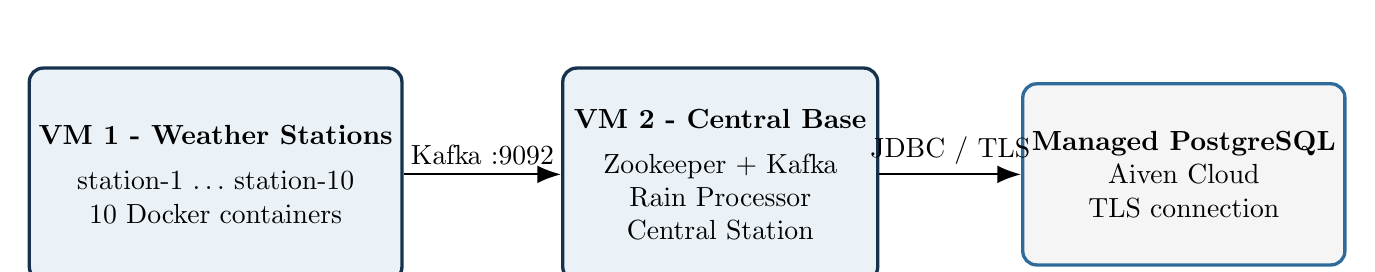
\begin{tikzpicture}[
    node distance=1.5cm,
    vm/.style={draw=navy, very thick, rounded corners=5pt, fill=lightblue,
               minimum width=4.0cm, minimum height=2.7cm, align=center},
    cloud/.style={draw=blueaccent, very thick, rounded corners=5pt, fill=gray!8,
                  minimum width=3.2cm, minimum height=2.3cm, align=center},
    arrow/.style={-{Latex[length=3mm]}, thick}
]
    \node[vm] (vm1) {\textbf{VM 1 - Weather Stations}\\[0.15cm]
                      station-1 $\ldots$ station-10\\10 Docker containers};
    \node[vm, right=2cm of vm1] (vm2) {\textbf{VM 2 - Central Base}\\[0.15cm]
                      Zookeeper + Kafka\\Rain Processor\\Central Station};
    \node[cloud, right=1.8cm of vm2] (aiven) {\textbf{Managed PostgreSQL}\\Aiven Cloud\\TLS connection};
    \draw[arrow] (vm1) -- node[above]{Kafka :9092} (vm2);
    \draw[arrow] (vm2) -- node[above]{JDBC / TLS} (aiven);
\end{tikzpicture}%
}
\caption{Bonus cloud deployment topology.}
\end{figure}

\subsection{Machine and Provider Details}
The repository contains a complete deployment procedure, but the actual provider, instance sizes, IP addresses, and managed database endpoint must be replaced with the values used during the final deployment before submission.

\begin{table}[H]
\centering
\caption{Cloud deployment details - replace placeholders with actual deployment values.}
\begin{tabularx}{\textwidth}{l l l l X}
\toprule
\textbf{Role} & \textbf{Provider} & \textbf{Size} & \textbf{vCPU/RAM} & \textbf{OS / Endpoint} \\
\midrule
Stations VM & [Provider] & [Size] & [vCPU/RAM] & Ubuntu [version], [IP] \\
Central VM & [Provider] & [Size] & [vCPU/RAM] & Ubuntu [version], [IP] \\
Database & Aiven Cloud & [Plan] & Managed & PostgreSQL [version], [host:port] \\
\bottomrule
\end{tabularx}
\end{table}

\subsection{Network Configuration}
The intended network policy follows least privilege. SSH port 22 is restricted to the administrator address. Kafka port 9092 on the Central VM is reachable only from the Weather Stations VM. The managed PostgreSQL service permits database access only from the required VM addresses. The central station connects using TLS with \texttt{DB\_SSLMODE=require}.

A key cloud-specific Kafka setting is \texttt{advertised.listeners}. The broker advertises an address that the remote Weather Stations VM can actually reach; otherwise the producer may contact the bootstrap address successfully but fail after Kafka metadata discovery redirects it to an unreachable internal hostname.

\subsection{Deployment Procedure}
The Central VM builds and runs Kafka, Zookeeper, the Rain Processor, and the Central Station through \texttt{cloud/docker-compose.central.yml}. Database parameters are loaded from a restricted \texttt{central.env} file with mode 600 rather than being committed to the repository.

The Weather Stations VM builds the weather station image, generates a Compose file containing ten station services with distinct IDs, and points all stations to the remote Kafka broker on the Central VM.

\begin{lstlisting}[language=bash,caption={Representative Central VM deployment commands.}]
sudo apt update
sudo apt install -y docker.io docker-compose-plugin git

git clone <repository-url>
cd distributed-weather-monitoring-system

docker build -t rain-processor:1.0.0  -f rain-processor/Dockerfile .
docker build -t central-station:1.0.0 -f central-station/Dockerfile .

cp cloud/central.env.example central.env
chmod 600 central.env
# Fill CENTRAL_VM_IP and managed DB credentials.

docker compose --env-file central.env \
  -f cloud/docker-compose.central.yml up -d
\end{lstlisting}

\begin{lstlisting}[language=bash,caption={Representative Weather Stations VM deployment commands.}]
sudo apt update
sudo apt install -y docker.io docker-compose-plugin git

git clone <repository-url>
cd distributed-weather-monitoring-system

docker build -t weather-station:1.0.0 -f weather-station/Dockerfile .
export KAFKA_BOOTSTRAP_SERVERS=<CENTRAL_VM_IP>:9092
./cloud/stations-compose.sh 10 "$KAFKA_BOOTSTRAP_SERVERS"
docker compose -f docker-compose.stations.yml up -d
\end{lstlisting}

% ================================================================
\section{Challenges and Lessons Learned}
% ================================================================
The implementation highlights several practical issues that are common in distributed systems:
\begin{itemize}
    \item \textbf{Random simulation must remain measurable.} Incrementing \texttt{s\_no} before the drop decision creates an observable ground truth for dropped-message analysis.
    \item \textbf{Partition keys affect ordering.} Using \texttt{station\_id} as the Kafka key preserves order for readings from the same station.
    \item \textbf{Persistence and offset commits must be coordinated.} Committing the database before Kafka offsets prevents acknowledged data from being lost, while database uniqueness constraints absorb replayed records.
    \item \textbf{Batching trades latency for throughput.} A 5000-record threshold is combined with a time-based flush so the system remains responsive during low traffic while still reducing I/O under higher load.
    \item \textbf{Stable identity matters in orchestration.} A StatefulSet provides deterministic station identities without duplicating Kubernetes manifests.
    \item \textbf{Secrets should be externalized.} Environment variables, Kubernetes Secrets, and restricted cloud environment files keep sensitive credentials out of application source code.
    \item \textbf{Cloud Kafka requires correct listener advertisement.} Remote clients must receive a broker address that is routable from their machine after Kafka metadata discovery.
\end{itemize}

% ================================================================
\section{Conclusion}
% ================================================================
This project successfully implements a complete distributed weather monitoring pipeline for the Net Centric Computing lab. Ten mock weather stations continuously produce structured readings, intentional message drops are measurable through sequence gaps, Kafka provides the communication backbone, and a stateful Kafka Streams processor generates rain alerts when humidity exceeds 70\%.

The central station persists readings efficiently using batched PostgreSQL writes and manual Kafka offset commits. Database constraints provide idempotent recovery behavior, while SQL analysis validates battery distribution, message-drop rate, latest station state, and rain-alert consistency. The application is containerized and deployed using Kubernetes with stable weather-station identities, persistent database storage, centralized configuration, and separate secret management. The cloud bonus architecture further demonstrates how the same services can be split across independent machines and connected to a managed PostgreSQL service.

Overall, the lab demonstrates the main concerns of a real distributed streaming system: asynchronous messaging, partitioning and ordering, stream processing, persistence, fault-aware delivery semantics, containerization, orchestration, remote networking, and secure configuration management.

\end{document}
